\section{Experiments}
\label{sec:experiments}

In this section, we will evaluate selected LVLMs, detail evaluation metrics and
discuss the results. 
% LVLMs we selected to evaluate,
% related

\subsection{Large Vision-Language Models}
\label{sec:lvlm}

We evaluated a selection of recent representative open-source and closed-source LVLMs in this paper, including InstructBLIP-7B \cite{dai2023instructblip}, Qwen-VL-Chat \cite{bai2023qwenvl}, LLaVA-v1.5-7B and LLaVA-v1.5-13B \cite{liu2023improved}, mPLUG-Owl-2 \cite{ye2023mplug}, ShareGPT4V-7B and ShareGPT4V-13B \cite{chen2023sharegpt4v}, GPT-4V and GPT-4o \cite{openai2023gpt4}. 
A brief introduction of these models is in Appendix C. % \ref{sec:lvlms}.
These open-source models are deployed on a machine with four GeForce RTX 2080 Ti GPUs and a machine with one GeForce RTX 3090 GPU.

%  \KZ{because ...}
% Table \ref{tab:lvlms} shows an overview of the design of different LVLMs.

% We select the following representative LVLMs for evaluation:

% \begin{itemize}
%     \item \textbf{InstructBLIP} \cite{dai2023instructblip} builds upon BLIP-2 \cite{li2023blip}. 
%     % and restructures 26 publicly available datasets into an instructional tuning format and uses 13 held-in datasets for instruction tuning. 
%     It consists of an image encoder, an LLM, and a Query Transformer (Q-Former). 
%     During instruction tuning, only the Q-Former is updated. We use ``blip2-vicuna-instruct'' for testing.
%     \item \textbf{Qwen-VL-Chat} \cite{bai2023qwenvl} is a instruction-tuned VL chatbot based on Qwen-VL. 
%     % Its training process consists of two stages of pre-training and a final stage of instruction fine-tuning. 
%     As for architecture, it consists of a vision encoder, a LLM, and position-aware vision-language adapter. We test ``Qwen-VL-Chat''.
%     \item \textbf{LLaVA v1.5} \citep{liu2023improved} is an upgraded version of LLaVA  \cite{liu2023llava}. 
%     % LLaVA connects a vision encoder and LLM for general-purpose visual and language understanding. 
%     It is instruction-tuned on the language-image instruction-following data generated by language-only GPT-4 \cite{openai2023gpt4}. 
%     By using CLIP-ViT-L-336px with an MLP projection and adding academic-task-oriented VQA data with simple response formatting prompts, LLaVA v1.5 achieves better performance. 
%     ``llava-v1.5-7b'' and ``llava-v1.5-13b'' are tested.
%     \item \textbf{mPLUG-Owl-2} \cite{ye2023mplug} mainly comprises a fundamental vision encoder, a visual abstractor, and a language decoder. 
%     % It also adopts a two-stage training strategy, comprising pre-training and visual instruction tuning. 
%     We test ``mplug-owl2-llama2-7b''. 
%     \item \textbf{ShareGPT4V} \cite{chen2023sharegpt4v} follows the design of LLaVA v1.5.
%     % 1.2 million
%     % ShareGPT4V dataset
%      They incorporate a large-scale resource featuring highly descriptive captions into both the pre-training and supervised fine-tuning phases of ShareGPT4V model.
%     % The model shows remarkable performance across a majority of the multi-modal benchmarks.
%     We test``ShareGPT4V-7B'' and ``ShareGPT4V-13B''.
%     \item \textbf{GPT-4V} \citep{openai2023gpt4} is one of the most powerful LVLMs in the world developed by OpenAI. The version of ``gpt-4-vision-preview'' is tested.
% \end{itemize}


% \begin{table}
%     \centering
%     \small
%     \begin{tabular}{lll}
%     \hline
%     \textbf{Model} & \thead{\textbf{Visual Encoder} } & \thead{\textbf{Language Model}}\\ % \\ \textbf{Accuracy}
%     \hline
%     InstructBLIP-7B  & EVA-CLIP ViT-g & Vicuna-7B \\
%     Qwen-VL-Chat & OpenCLIP ViT-G & Qwen-7B \\
%     LLaVA-v1.5-7B  & CLIP ViT-L & Vicuna-7B \\
%     LLaVA-v1.5-13B & CLIP ViT-L & Vicuna-13B \\
%     mPLUG-Owl-2 & CLIP ViT-L & LLaMA-7B \\
%     % Otter  &  &   \\
%     % CogVLM & 0 & & & & & & & & \\
%     ShareGPT4V-7B & CLIP ViT-L & Vicuna-7B \\
%     ShareGPT4V-13B & CLIP ViT-L & Vicuna-13B \\
%     % Monkey &  &  \\
%     GPT-4V & \multicolumn{1}{c}{--}  & \multicolumn{1}{c}{--} \\
%     \hline
%     \end{tabular}
%     \caption{\label{tab:lvlms}
%     LVLMs evaluated in this paper.
%     }
% \end{table}
\subsection{CogBench Evaluation Strategy}

% ShareGPT-4V 
\paragraph{Evaluation for Description Task}

Here we consider model performance at two levels: low-level Recognition ability and high-level Cognition ability. 
Evaluation metrics for both levels are calculated using recall scores, referred to as Recognition Score and Cognition Score, respectively.
% \KZ{Instead of calling them recognition vs. cognition, I suggest calling them
% ``hard coverage'' and ``soft coverage''.} 
% \XJ{seems we did not emphasis soft and hard?}

% \subsubsection*{Recognition}
% \KZ{No point having 3rd level of sections.}
% For the Recognition part, we calculate recall score based on [Entities] as the Recognition Score. 
% We use the following method to calculate recall score:
% For the Recognition part, the recall score
% \textbf{Recognition} \quad
% \paragraph{Recognition}
The \textbf{Recognition Score} is calculated as the ratio of the number of recognized [Entities] to the number of annotated [Entities] in all images.
%  which is referred to as the Recognition Score.
First, we use SpaCy\footnote{https://spacy.io/} to extract nouns from the model generated description, and then calculate cosine similarity between embeddings\footnote{Implemented with sentence-transformers package (https://www.sbert.net) and \textit{all-mpnet-base-v2} is adopted as the model to encode [Entities] and nouns.} of annotated [Entities] and extracted nouns. 
% Sentence-BERT \cite{reimers-2019-sentence-bert} is adopted to encode the nouns and [Entities]. 
For each entity, if the cosine similarity score between the entity and any noun is greater than a threshold (0.6 in this paper), we consider the entity is recognized by the model. 
% The recall score of an image is the ratio of the number of recognized entities to the number of entities in the image.
% The micro-average score is finally calculated as the overall Recognition Score. 
% of each model on Description task.
% \MY{It's better to discuss the results with respect to the ``cognitive capability checklist'' at first, you can group them into recognition and cognition, but still stick to the framework you proposed. You can group in the annotation section in a more obvious way, saying that your recognition includes xxx while cognition includes xxx}

% For the Sentence-BERT adopted for evaluation, we implemented with sentence-transformers \footnote{https://www.sbert.net} and use \textit{all-mpnet-base-v2} as the model.

% \subsubsection{Cognition}

% For the Cognition part, 
% \paragraph{Cognition} 
% We evaluate the cognitive reasoning abilities of LVLMs from the eight aspects as we annoated.
% We calculate the Cognition Score of each CoR type to evaluate the performance of models on different reasoning capabilities.
% \MY{eight CoRs spanning from time to mental state reasoning?}\XJ{Yes}
For \textbf{Cognition Score}, we calculate both scores for each of the eight cognitive reasoning abilities and an overall score using GPT-4~\cite{openai2023gpt4}. To enhance objectivity and granularity, GPT-4 is utilized for a binary classification task to assess if generated descriptions include the semantics of annotated CoRs, as detailed in Appendix D. %  \ref{sec:cogid_eval_prompt}
The CoR scores for each type of reasoning capability are then used to compute a recall score for each respective type. 
The overall Cognition Score is the sum of all CoR scores divided by the total number of CoRs.
% \MY{I condensed this part, please check. you might have space for other stuff now. i.e. enlarging some figures}
%first calculate a score for each of the eight cognitive reasoning abilities, and then compute an overall score.
%We use GPT-4 \cite{openai2023gpt4} to help calculate the Cognition Score. To avoid the interpretability issues of GPT-based evaluation, instead of using a subjective evaluation method of directly comparing two descriptions, we use GPT-4 to perform a easier, more objective and fine-grained binary classification task, that is, judging whether the generated description contains the semantics of annotated CoRs.Details and prompts of this GPT-based evaluation are shown in Appendix \ref{sec:cogid_eval_prompt}.
% we use GPT to perform a easier and more fine-grained task instead of a coarse-grained evaluation task to directly evluate the quality of the generated description. 
% For CoR types other than [Event Relationship Reasoning], we task GPT with determining whether the conclusion in each CoR is mentioned in the description. 
% For [Event Relationship Reasoning], we task GPT with determining whether the causal relationship between events (i.e. the whole CoR), as annotated, is present in the description.
% Prompts of the two subtasks mentioned above are shown in Appendix \ref{sec:cogid_eval_prompt}.
% \begin{figure}
%     \begin{tcolorbox}
%         % [title = {Reasoning Eval},
%         [colframe = blue!30!white,
%         colback = blue!2!white,
%         colbacktitle = blue!10!white,
%         colupper = black, collower = yellow!75!red,
%         coltitle = black!90!white]
%         \small
%         \textit{
%         Given a \textcolor{blue}{<DESCRIPTION>} and some \textcolor{green}{<KEY POINT>s}, please tell me if the description explicitly present the exact or similar semantic meaning of each key points. Note that instead of reasoning about whether each key point is possibly correct based on the description, you only need to determine whether the description mentions semantic information in the key point. If there is ``or'' in the key point, you just need to determine if the description mentions any of the situations listed in the key point. Assign a score of 0 or 1 to each key point, where 0 represents NO and 1 represents YES.} \\
%         \textit{\textcolor{blue}{<DESCRIPTION>:}} \\
%         \textit{\textcolor{blue}{\{Description generated by models.\}}} \\
%         \textit{\textcolor{green}{<KEY POINT>:}} \\
%         \textit{\textcolor{green}{1. \{Annotated key point.\}}} \\
%         \textit{\textcolor{green}{2. \{Annotated key point.\}}} \\
%         \textit{\textcolor{green}{3. \{Annotated key point.\}}} \\
%         \textit{...} \\
%         \textit{Please write your answers in this format:} \\
%         \textit{1. [ ]  2. [ ]  3. [ ]  ...} \\
%     \end{tcolorbox}
%     \caption{Evaluation of Reseasoning types.}
%     \label{fig:eval}
% \end{figure}
% After obtaining the score of each CoR, we calculate the Cognition Score by summing up the scores of all CoRs and dividing by the number of CoRs in the image.
% We calculate the Cognition Score of each CoR type to evaluate the performance of models on different reasoning capabilities.
% Finally, we calculate micro-average score as the overall Cognition Score of each model on Description task.
%After obtaining the score of each CoR, we calculate a recall score for each reasoning capabilities. The overall Cognition Score is calculated by summing up the scores of all CoRs and dividing by the total number of CoRs.
% The effectiveness analysis of GPT-based cognition evaluation is shown in Appendix \ref{sec:eval_gpt_eval}.

% Note that it is similar to \citet{chan-etal-2023-clair}.


% Besides, traditional evaluation metrics are we also adopted as reference. We use BLEU-4, METEOR, ROUGE-L, CIDEr-D, SPICE, and BERTScore as evaluation metrics.


\paragraph{Evaluation for VQA Task}

For Multiple-Choice Questions in VQA task, we use accuracy as the evaluation metric. 
As questions are generated based on CoRs, we can also calculate the accuracy for both each reasoning capability and the overall cognition capability.

\subsection{Results of Description Task}
% \KZ{To make space, this whole subsection can be simplified a lot. Many statements about the comparisons are not that useful. Basically all you can say is that there's a gap in  performance in all these models, even for GPT4, and our benchmark quite hard. That's it!}
% As mentioned earlier, we consider both recognition and cognition ability of LVLMs in CogID task.

% For fair comparison, we use the following prompt for LVLMs to generate image description:

We prompt the selected LVLMs with the following instruction to obtain detailed descriptions about images in CogBench:
``\texttt{Describe this image in detail.}''
We evaluate the performance of LVLMs on Description task in terms of both recognition and cognition ability.
As a reference, we also calculated traditional image captioning evaluation metrics by comparing annotated reference description and model-generated description, and details are shown in Appendix E. %  \ref{sec:cap_eval}

\subsubsection{Recognition}



Table \ref{tab:rec_score} shows Recognition Scores of models on Description task.
GPT-4o achieves the best performance in terms of recognition, which means it can recognize and describe more entities.
Besides, GPT-4o and GPT-4V are significantly better than other open-source LVLMs, indicating these open-source LVLMs still have some room for development before reaching the recognition capability of GPT-4.
%  there is some room for improvement in recognition ability of open-source LVLMs before reaching the capability of GPT-4.
ShareGPT4V-7B and ShareGPT4V-13B achieves better performance than other open-source LVLMs.
As it follows the design of LLaVA v1.5, one possible reason is that ShareGPT4V uses a high-quality image-text dataset featuring highly descriptive captions for training, which makes it describe more entities shown in images. 
% This shows the importance of high-quality dataset for improving recognition ability of LVLMs in image description.
GPT-4o, while top-performing, still misses many entities, suggesting room for improvement even on recognition capability.
% Though GPT-4o achieves the best performance, there are still a lot of entities that are not recognized by it, indicating a room for improvement.\MY{for concise purpose: GPT-4o, while top-performing, still misses many entities, suggesting room for improvement even on recognition capability.}

%  indicating that there is still a gap between the recognition ability of LVLMs and human beings.

% % based on 20240124_94
% \begin{table}
%     \centering
%     \small
%     \begin{tabular}{lc}
%     \hline
%     \textbf{Model} & \textbf{Recognition Score}\\ % \\ \textbf{Accuracy}
%     \hline
%     InstructBLIP-7B  & 0.516 \\
%     Qwen-VL-Chat & 0.553  \\
%     LLaVA-v1.5-7B  & 0.526 \\
%     LLaVA-v1.5-13B & 0.526  \\
%     mPLUG-Owl-2 & 0.487  \\
%     % CogVLM & 0 & & & & & & & & \\
%     ShareGPT4V-7B & 0.578 \\
%     ShareGPT4V-13B & 0.613 \\
%     % Monkey &  &  \\
%     GPT-4V & 0.774 \\
%     \hline
%     \end{tabular}
%     \caption{
%     \label{tab:rec_score}
%     Recognition Score of models on CogID task.
%     }
% \end{table}

% % based on 20240204_95, macro average
% \begin{table}
%     \centering
%     \small
%     \begin{tabular}{lc}
%     \hline
%     \textbf{Model} & \textbf{Recognition Score}\\ % \\ \textbf{Accuracy}
%     \hline
%     InstructBLIP-7B  & 0.515 \\
%     Qwen-VL-Chat & 0.551  \\
%     LLaVA-v1.5-7B  & 0.525 \\
%     LLaVA-v1.5-13B & 0.525  \\
%     mPLUG-Owl-2 & 0.484  \\
%     % CogVLM & 0 & & & & & & & & \\
%     ShareGPT4V-7B & 0.579 \\
%     ShareGPT4V-13B & 0.613 \\
%     % Monkey &  &  \\
%     GPT-4V & 0.772 \\
%     \hline
%     \end{tabular}
%     \caption{
%     \label{tab:rec_score}
%     Recognition Score of LVLMs on CogID task.
%     }
% \end{table}

% % based on 20240204_95, micro average
% \begin{table}
%     \centering
%     \small
%     \setlength{\tabcolsep}{2.5pt} 
%     \begin{tabular}{lc}
%     \hline
%     \textbf{Model} & \textbf{Recognition Score}\\ % \\ \textbf{Accuracy}
%     \hline
%     InstructBLIP-7B  & 0.498 \\
%     Qwen-VL-Chat & 0.541  \\
%     LLaVA-v1.5-7B  & 0.512 \\
%     LLaVA-v1.5-13B & 0.516  \\
%     mPLUG-Owl-2 & 0.479  \\
%     % CogVLM & 0 & & & & & & & & \\
%     ShareGPT4V-7B & 0.574 \\
%     ShareGPT4V-13B & 0.602 \\
%     % Monkey &  &  \\
%     GPT-4V & 0.766 \\
%     \hline
%     Human & 0.944 \\
%     \hline
%     \end{tabular}
%     \caption{
%     \label{tab:rec_score}
%     Recognition score of LVLMs on Description task. 
%     For reference, the Recognition Score of Human is calculated based on the annotated [Description] in CogBench as an estimate of an upper limit score. 
%     \KZ{Not clear how you
%     get the human scores. How many people did you use, 
%     their age/sex/health condition?}}
% \end{table}

% based on 20240204_95, micro average, (2)
% \begin{table}
%     \centering
%     \small
%     \setlength{\tabcolsep}{2.5pt} 
%     \begin{tabular}{lc}
%     \hline
%     \textbf{Model} & \thead{\textbf{Recognition Score} }\\ % \\ \textbf{Accuracy}
%     \hline
%     InstructBLIP-7B  & 0.50 \\  %0.498
%     Qwen-VL-Chat & 0.54  \\ % 0.541
%     LLaVA-v1.5-7B  & 0.51 \\  % 0.512
%     LLaVA-v1.5-13B & 0.52  \\ % 0.516
%     mPLUG-Owl-2 & 0.48  \\ % 0.479
%     % CogVLM & 0 & & & & & & & & \\
%     ShareGPT4V-7B & 0.57 \\ % 0.574
%     ShareGPT4V-13B & 0.60 \\ % 0.602
%     % Monkey &  &  \\
%     GPT-4V & 0.77 \\ % 0.766
%     \hline
%     Human & 0.94 \\ % 0.944
%     \hline
%     \end{tabular}
%     \caption{
%     \label{tab:rec_score}
%     Recognition score of LVLMs on Description task. 
%     For reference, the Recognition Score of Human is calculated based on the annotated [Description] in CogBench as an estimate of an upper limit score. 
%     % \KZ{Not clear how you
%     % get the human scores. How many people did you use, 
%     % their age/sex/health condition?}
%     }
% \end{table}

\begin{table}
% \begin{wraptable}{r}{0.45\textwidth}
    \centering
    \small
    \setlength{\tabcolsep}{2.5pt} 

    \begin{tabular}{lc}
    \hline
    \textbf{Model} & \thead{\textbf{Recognition Score} }\\ % \\ \textbf{Accuracy}
    \hline
    InstructBLIP-7B  & 0.40 \\  %0.498
    Qwen-VL-Chat & 0.42 \\ % 0.541
    LLaVA-v1.5-7B  & 0.40 \\  % 0.512
    LLaVA-v1.5-13B & 0.41 \\ % 0.516
    mPLUG-Owl-2 &  0.37 \\ % 0.479
    % CogVLM & 0 & & & & & & & & \\
    ShareGPT4V-7B & 0.47 \\ % 0.574
    ShareGPT4V-13B & 0.49 \\ % 0.602
    % Monkey &  &  \\
    GPT-4V & 0.67 \\ 
    GPT-4o & 0.72 \\ 
    \hline
    Oracle & 0.93 \\ % 0.944
    \hline
    \end{tabular}
    \caption{
        \label{tab:rec_score}
        Recognition score of LVLMs on Description task. 
        For reference, the Recognition Score of Oracle is calculated based on the annotated [Description] in CogBench as an estimated upper bound. 
        % \KZ{You should give the formula for calculating the Oracle score.}
        % \XJ{The difference between Oracle and others is input instead of the formula. They share the same formula.}
        }
\end{table}
% \end{wraptable}


\subsubsection{Cognition}



% \KZ{This para is very verbose and many of the comparisons are not meaningful. What's the point of saying X is better than Y, when you don't know why?} 
Table \ref{tab:cogid} shows Cognition Scores of LVLMs on Description task. 
Similarly, GPT-4o achieves the best performance and there is a large performance gap between GPT-4 and other open-source models. 
For open-source models, Qwen-VL-Chat achieves the best performance.
% Though ShareGPT4V achieves better recognition performance than other open-source LVLMs, it's cognition performance does not show a significant improvement compared with all other open-source models.
% However, its cognitive abilities are indeed slightly stronger than LLaVA-v1.5.
In terms of different reasoning capabilities, all of the LVLMs show better performance on [Location Reasoning] than others, which is probably because it is a kind of relatively lower-level reasoning.
Differently, for [Event Reasoning], [Event Relationship Reasoning], and [Next Moment Event Reasoning], all of the open-source LVLMs show very low performance, indicating they almost do not understand the story in the images at all.
The significantly large performance gap on these three kinds of reasoning types between GPT-4 and open-source LVLMs could be a manifestation of the capabilities emerging in GPT-4.
Though GPT-4o achieves the best performance, there is also a huge gap between its ability and the Oracle, and the gap is obviously larger than that of recognition scores.
This indicates that LVLMs still have a lot of room for development in terms of cognitive abilities.

% indicating CogID task is still a challenging problem for LVLMs.

% Comparing Table \ref{tab:rec_score} and Table \ref{tab:cogid}, we can observe the gap between the recognition ability and cognition ability of LVLMs.


% indicates that improving cognition ability of LVLMs is still a challenging problem.

% % evaluated by ChatGPT
% \begin{table*}
%     \centering
%     \small
%     \begin{tabular}{lccccccccc}
%     \hline
%     \textbf{Model} & \thead{\textbf{Time} } & \thead{\textbf{Location} } & \thead{\textbf{Character} } &  \thead{\textbf{Character}\\ \textbf{Relationship} } & \thead{\textbf{Event} } & \thead{\textbf{Event} \\ \textbf{Relationship} } & \thead{\textbf{Mental} \\ \textbf{State} } & \thead{\textbf{Next}\\ \textbf{Moment} \\ \textbf{Event} } & \thead{\textbf{Overall} } \\ % \\ \textbf{Accuracy}
%     \hline
%     InstructBLIP-7B  & 0.174 & 0.641 & 0.262 & 0.376 & 0.143 & 0.053  & 0.109 & 0.289 & 0.228  \\
%     Qwen-VL-Chat & 0.391 & 0.615 & 0.333 & 0.347 & 0.180  & 0.147 & 0.091 & 0.289 & 0.259 \\
%     LLaVA-v1.5-7b  & 0.130 & 0.538 & 0.238 & 0.307 & 0.111 & 0.065 & 0.109 & 0.270  & 0.198  \\
%     LLaVA-v1.5-13b & 0.043 & 0.590 & 0.333 & 0.386 & 0.086 & 0.041 & 0.127 & 0.289 & 0.208 \\
%     mPLUG-Owl-2 & 0.217 & 0.500 & 0.143 & 0.287 & 0.139 & 0.071 & 0.109 & 0.226 & 0.192 \\
%     % ShareGPT4V-7B & 0.261 & 0.577 & 0.286 & 0.347 & 0.119 & 0.029 & 0.091 & 0.277 & 0.208 \\
%     % CogVLM & 0 & & & & & & & & \\
%     ShareGPT4V-7B & 0.217 & 0.551 & 0.262 & 0.347 & 0.139 & 0.024 & 0.091 & 0.277 & 0.208 \\
%     ShareGPT4V-13B & 0.304 & 0.603 & 0.262 & 0.386 & 0.119 & 0.047 & 0.109 & 0.302 & 0.224 \\
%     % Monkey &  &  &  &  &  &  &  & &  \\
%     GPT-4V & 0.478 & 0.769 & 0.524 & 0.426 & 0.381 & 0.229 & 0.236 & 0.619 & 0.435 \\
%     \hline
%     \end{tabular}
%     \caption{\label{tab:cogid}
%     Cognitive Scores of models on CogID task. Evaluated by ChatGPT.
%     }
% \end{table*}


\begin{table*}[h!]
    \centering
    \small
    \setlength{\tabcolsep}{1.5pt} 

    \begin{tabular}{lccccccccc}
    \hline
    \textbf{Model} & \thead{\textbf{Time} } & \thead{\textbf{Location} } & \thead{\textbf{Character} } &  \thead{\textbf{Character}\\ \textbf{Relationship} } & \thead{\textbf{Event} } & \thead{\textbf{Event} \\ \textbf{Relationship} } & \thead{\textbf{Next}\\ \textbf{Moment} \\ \textbf{Event} } & \thead{\textbf{Mental} \\ \textbf{State} } & \thead{\textbf{Overall} } \\ % \\ \textbf{Accuracy}
    \hline
    InstructBLIP-7B  & 0.15 & 0.54 & 0.25 & 0.30 & 0.10 & 0.05 & 0.02 & 0.17 & 0.17 \\
    Qwen-VL-Chat  & 0.28 & 0.57 & 0.28 & 0.26 & 0.14 & 0.12 & 0.04 & 0.13 & 0.19 \\
    LLaVA-v1.5-7B  & 0.09 & 0.45 & 0.15 & 0.18 & 0.09 & 0.05 & 0.02 & 0.13 & 0.13 \\
    LLaVA-v1.5-13B  & 0.13 & 0.49 & 0.18 & 0.24 & 0.10 & 0.05 & 0.04 & 0.16 & 0.15 \\
    mPLUG-Owl-2  & 0.06 & 0.48 & 0.24 & 0.21 & 0.08 & 0.04 & 0.02 & 0.14 & 0.14 \\
    % CogVLM & 0 & & & & & & & & \\
    ShareGPT4V-7B  & 0.19 & 0.60 & 0.21 & 0.22 & 0.10 & 0.04 & 0.03 & 0.15 & 0.16 \\
    ShareGPT4V-13B  & 0.23 & 0.57 & 0.24 & 0.26 & 0.12 & 0.07 & 0.03 & 0.14 & 0.17 \\
    % Monkey &  &  &  &  &  &  &  & &  \\
    GPT-4V & 0.43 & 0.71 & 0.47 & 0.24 & 0.35 & 0.31 & 0.10 & 0.46 & 0.37 \\
    GPT-4o & 0.51 & 0.77 & 0.55 & 0.37 & 0.44 & 0.39 & 0.15 & 0.40 & 0.43 \\
    \hline
    Oracle  & 0.92 & 0.98 & 0.94 & 0.81 & 0.98 & 0.92 & 0.90 & 0.92 & 0.93 \\
    \hline
    \end{tabular}
    \caption{\label{tab:cogid}
    Cognition Scores of LVLMs on Description task evaluated by GPT-4.
    For reference, the Cognition Score of Oracle is calculated based on the annotated [Description] in CogBench as an estimated upper bound. 
    % \KZ{Give the formula for calculating the oracle score.}
    }
\end{table*}

\subsubsection{Case Study of Description Task}

\begin{figure*}[th]
    \centering
    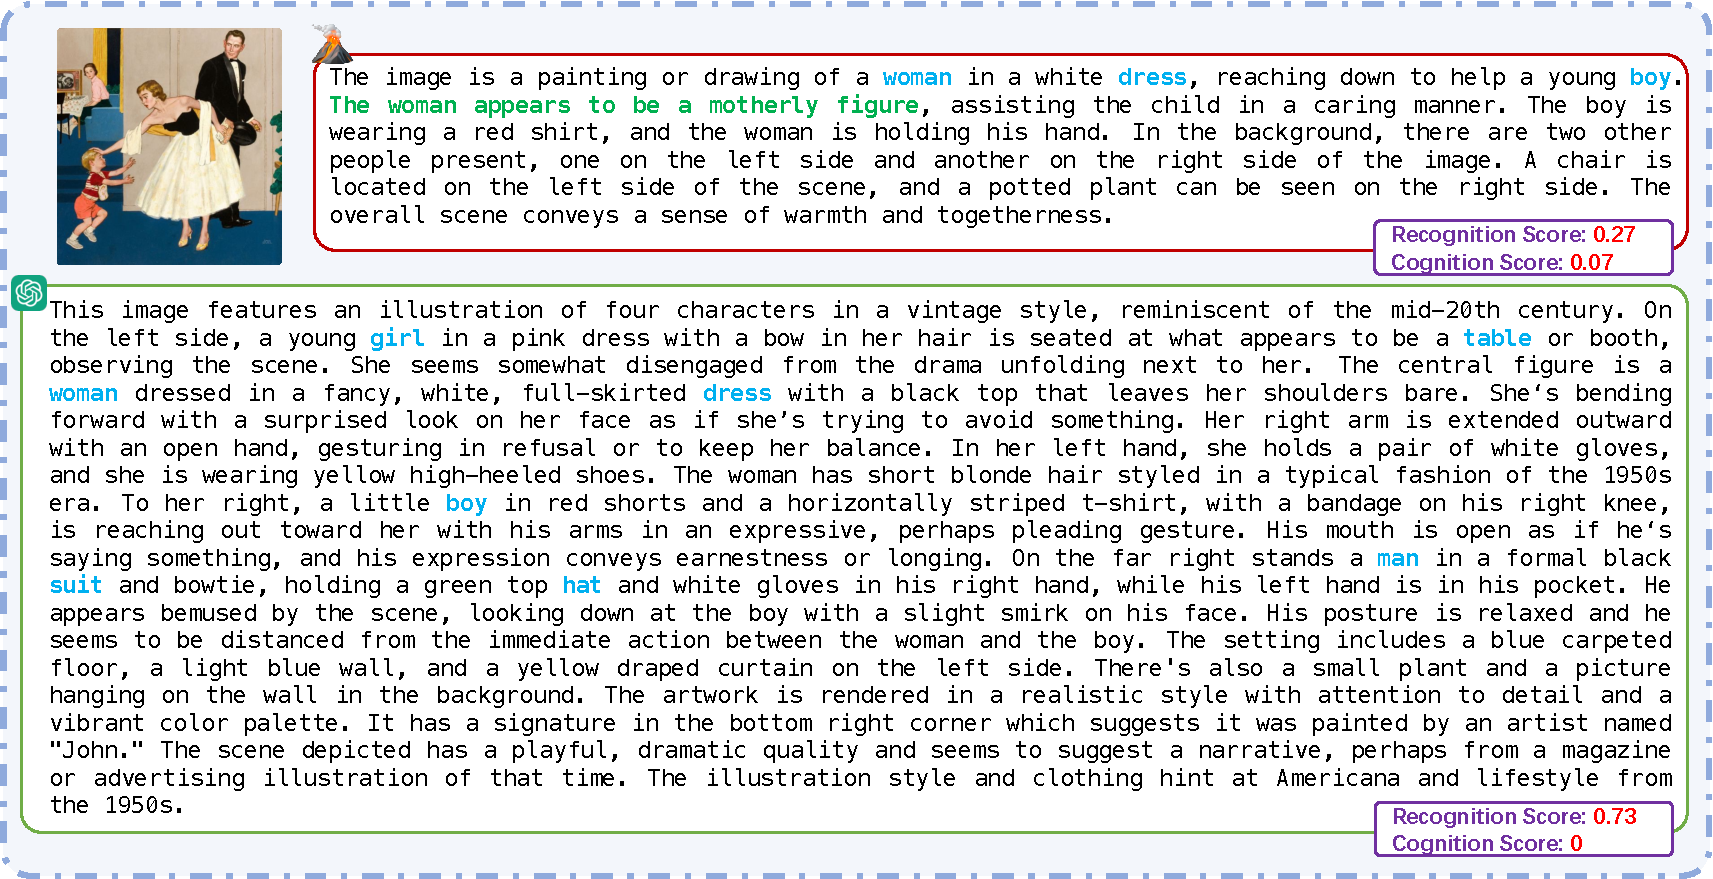
\includegraphics[width=0.95\textwidth]{figs/case_single3.pdf}
    \caption{Case study of the Description task. 
    A representative open-source LVLM LLaVA-v1.5-13B (red frame) and GPT-4V (green frame) are selected for analysis. 
    Recognized entities are marked in \textcolor{c3}{blue}, and CoRs are marked in \textcolor{c2}{green}.
    }
    \label{fig:case}
\end{figure*}

% \KZ{I think we don't need this case study, because this paper is not about
% the analysis of the existing LLMs. This paper is a benchmark dataset paper.} \MY{I thind we need case study but to show that our benchmark is reasonable and can reflect that models fail at certain aspects, not the purpose to entirely compare the models. To show that healthy humans have no problem while current LVLM are incapable}
% \MY{color certain text as you do in the figure?} (``\textcolor{c3}{boy}'', ``\textcolor{c3}{girl}'', ``\textcolor{c3}{man}'', ``\textcolor{c3}{woman}'', ``\textcolor{c3}{table}'', ``\textcolor{c3}{dress}'', ``\textcolor{c3}{hat}'', ``\textcolor{c3}{suit}'') the ``sofa'', ``television'', ``handbag''``\textcolor{c3}{boy}'', ``\textcolor{c3}{woman}'', and ``\textcolor{c3}{dress}''
Figure \ref{fig:case} shows a case of Description task.
In terms of recognition, GPT-4V shows a good performance by recognizing most annotated entities such as \texttt{boy, girl, man, woman, table, dress, hat, suit} and only fails to recognize \texttt{\textcolor{c3}{sofa, television, handbag}} .
LLaVA-v1.5-13B obviously recognizes fewer entities than GPT-4V, as it only recognizes \texttt{boy, woman, dress}.
However, GPT-4V fails to understand the story in the image and gets a 0 in terms of cognition.
This is because it neither clarifies the location nor the relationships between the characters, nor does it accurately depict the events occurring in the image, etc.
LLaVA-v1.5-13B is slightly better and successfully inferred that \texttt{\textcolor{c2}{the woman is the mother}}.
% In the second image, GPT-4V shows a better performance in terms of cognition. 
% It successfully inferred key information such as ``winter'', ``bus stop'', ``the man in the phone booth is happy'', etc. 
% However, it failed to infer the high-level event of ``the man is sheltering from the cold wind in the phone booth'' and the women's reaction to his behavior, etc.
% As for LLaVA-v1.5-13B, though it recognizes some entities but only inferred ``winter'' successfully, and has a low Cognition Score.
This case demonstrates that CogBench reveals current LVLMs falling short in recognition and cognition, with a gap remaining between their cognitive abilities and human levels.
% The case shows CogBench can reflect that current LVLMs fail at aspects like recognition and cognition and the cognitive abilities exhibited in the description still have some gap with the level of humans.\MY{rewrite suggestion: This case demonstrates that CogBench reveals current LVLMs falling short in recognition and cognition, with a gap remaining between their cognitive abilities and human levels.}

% \begin{figure*}[th]
%     \centering
%     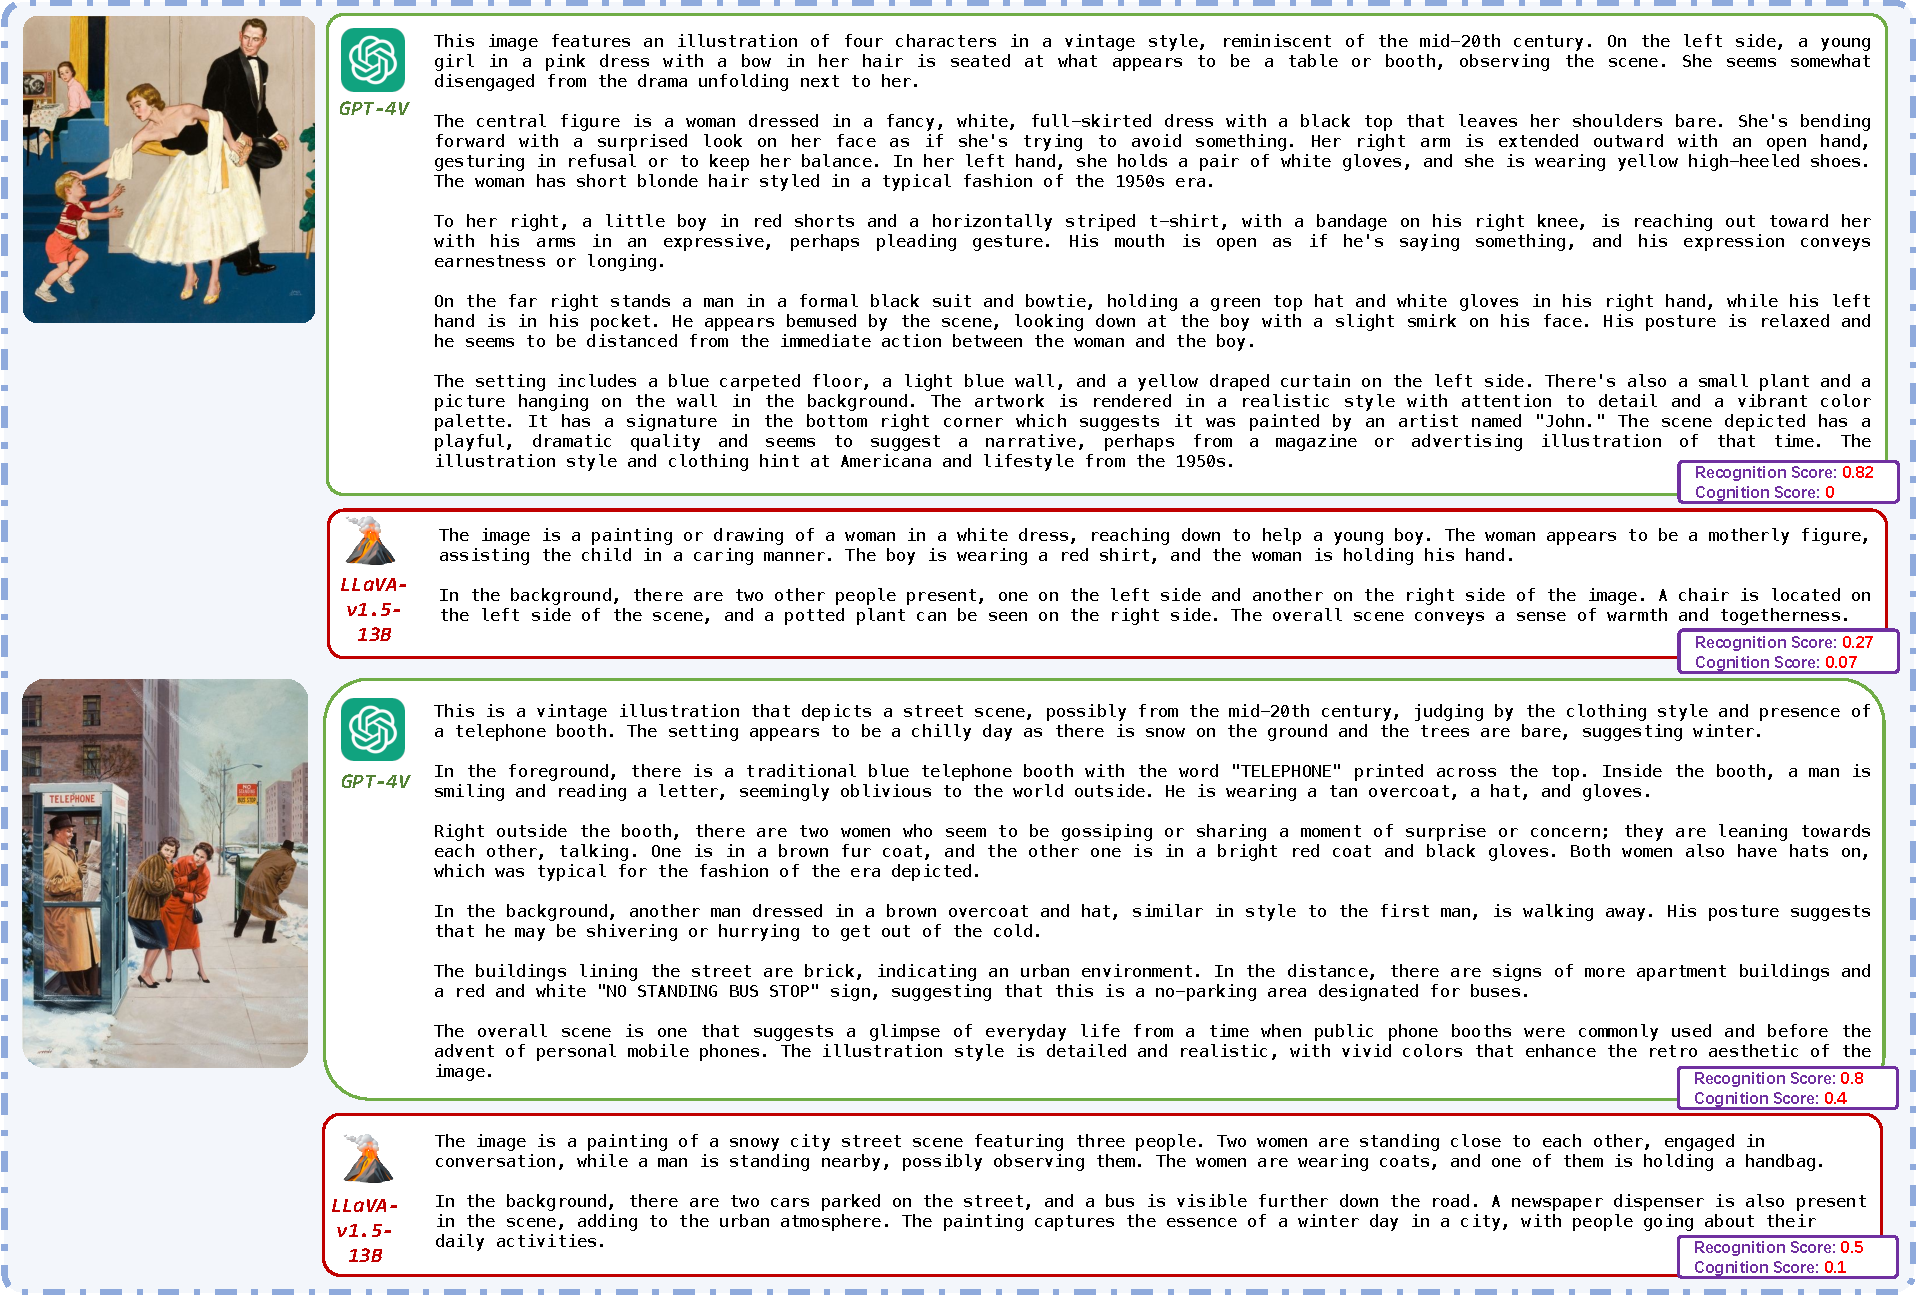
\includegraphics[width=0.95\textwidth]{figs/case2.pdf}
%     \caption{Case study of the Description task. GPT-4V and a representative open-source LVLM LLaVA-v1.5-13B is selected for analysis. \KZ{This pic takes
% too much space and should go into Appendix at least.}}
%     \label{fig:case}
% \end{figure*}



\subsubsection{Effectiveness Analysis of GPT-based Cognition Evaluation of Description Task}
% \label{sec:eval_gpt_eval}

% Considering the interpretability issues 

% after 20240204_95
\begin{table}[h!]
% \begin{wraptable}[8]{r}{0.35\textwidth}
    % \vspace*{-15pt}
    \centering
    \small

    \begin{tabular}{lc}
    \hline
    \textbf{Model} & \textbf{Accuracy}\\ % \\ \textbf{Accuracy}
    \hline
    ROUGE & 0.656 \\
    % ROUGE-paragraph & 0.567  \\
    BERTScore & 0.635 \\
    % BERTScore-paragraph & 0.620  \\
    BLEURT & 0.620 \\
    DeBERTa & 0.693 \\
    DocNLI  & 0.714 \\
    GPT-3.5 & 0.807 \\
    GPT-4 & 0.833 \\
    \hline
    \end{tabular}
    \caption{\label{tab:eval_metrics}
    CoR accuracy of evaluation methods.
    % Accuracy of different evaluation methods.\MY{CoR Accuracy of Evaluation Metrics?}
    }
\end{table}
% \end{wraptable}

% To prove the effectiveness of GPT-based evaluation, we manually annotated a subset by assigning 0/1 to CoRs of 20 images and use the subset to evaluate the performance of different evaluation methods.
% Table \ref{tab:eval_metrics} shows the accuracy of different evaluation methods on the subset.
% It can be seen that GPT-4 achieves the best performance, which indicates that GPT-based evaluation is generally consistent with human evaluation and thus effective for evaluating the performance of LVLMs on Description task.
%  \MY{consider: To validate GPT-based evaluation, we manually scored 0/1 on 20 images' CoRs and compared various methods' accuracy on this subset. Table \ref{tab:eval_metrics} reveals that GPT-4 offers the highest accuracy, demonstrating that GPT-based evaluation aligns well with human assessment and is effective for assessing LVLMs' performance on the Description task. Additional details on evaluation methods are available in Appendix \ref{sec:eval_gpt_eval}.}
To validate GPT-based cognition evaluation, we manually scored the CoRs of 20 images with a binary scale (0/1) and compared various evaluation methods' accuracy on this subset. 
Table \ref{tab:eval_metrics} reveals that GPT-4 offers the highest accuracy, demonstrating that GPT-based evaluation aligns well with human assessment. 
Therefore it is effective to assess LVLMs' performance on the Description task. 
Implementation details of evaluation methods beyond ChatGPT and GPT-4~\citep{lin2004rouge, bertscore, sellam2020bleurt, he2021deberta, yin-etal-2021-docnli} can be found in Appendix F. % \ref{sec:eval_gpt_eval}

%Additional details on evaluation methods are available in Appendix \ref{sec:eval_gpt_eval}.


% we manually scored 0/1 the CoRs of 20 images 
% % Details are shown in Appendix.
% % Besides, as the evaluation task is a fine-grained discriminative task, the interpretability problem of GPT can be alleviated to some extent.

% % before 20240204_95
% % \begin{table}
% %     \centering
% %     \small
% %     \begin{tabular}{lc}
% %     \hline
% %     \textbf{Model} & \textbf{Accuracy}\\ % \\ \textbf{Accuracy}
% %     \hline
% %     ROUGE  & 0.656 \\
% %     % ROUGE-paragraph & 0.567  \\
% %     BERTScore & 0.641 \\
% %     % BERTScore-paragraph & 0.620  \\
% %     BLEURT & 0.620 \\
% %     DeBERTa & 0.682 \\
% %     DocNLI  & 0.703 \\
% %     GPT-3.5 & 0.797 \\
% %     GPT-4 & 0.83 \\
% %     \hline
% %     \end{tabular}
% %     \caption{\label{tab:eval_metrics}
% %     Accuray of different evaluation methods on human evaluation.
% %     }
% % \end{table}

% % after 20240204_95
% \begin{table}
%     \centering
%     \small
%     \begin{tabular}{lc}
%     \hline
%     \textbf{Model} & \textbf{Accuracy}\\ % \\ \textbf{Accuracy}
%     \hline
%     ROUGE  & 0.656 \\
%     % ROUGE-paragraph & 0.567  \\
%     BERTScore & 0.635 \\
%     % BERTScore-paragraph & 0.620  \\
%     BLEURT & 0.620 \\
%     DeBERTa & 0.693 \\
%     DocNLI  & 0.714 \\
%     GPT-3.5 & 0.807 \\
%     GPT-4 & 0.849 \\
%     \hline
%     \end{tabular}
%     \caption{\label{tab:eval_metrics}
%     Accuray of different evaluation methods.
%     }
% \end{table}


\subsection{Results of VQA Task}

% this table is calculated based on 95 pics
\begin{table*}[h!]
    \centering
    \small
    \setlength{\tabcolsep}{1.5pt} 

    \begin{tabular}{lccccccccc}
    \hline
    \textbf{Model} & \thead{\textbf{Time} } & \thead{\textbf{Location} } & \thead{\textbf{Character} } &  \thead{\textbf{Character}\\ \textbf{Relationship} } & \thead{\textbf{Event} } & \thead{\textbf{Event} \\ \textbf{Relationship} } & \thead{\textbf{Next}\\ \textbf{Moment} \\ \textbf{Event} } & \thead{\textbf{Mental} \\ \textbf{State} } & \thead{\textbf{Overall} } \\ % \\ \textbf{Accuracy}
    \hline
    % InstructBLIP-7B & 0.56 & 0.65 & 0.49 & 0.48 & 0.36 & 0.38  & 0.44 & 0.43 & 0.44 \\  % this is reults based on generation
    InstructBLIP-7B & 0.60 & 0.71 & 0.49 & 0.55 & 0.40 & 0.37 & 0.47 & 0.48 & 0.47 \\
    Qwen-VL-Chat & 0.65 & 0.82 & 0.60 & 0.54 & 0.51  &  0.45 & 0.47 & 0.51 & 0.54 \\
    LLaVA-V1.5-7B & 0.58 & 0.81 & 0.54 & 0.55 & 0.46 & 0.45  & 0.54 & 0.53  & 0.53 \\
    LLaVA-V1.5-13B & 0.70 & 0.82 & 0.65 & 0.60 & 0.50 & 0.47 & 0.58 & 0.57 & 0.57 \\
    % CogVLM & 0 & & & & & & & & \\
    mPLUG-Owl-2 & 0.51  & 0.82  & 0.59 & 0.55 &  0.46 &  0.48 & 0.47 & 0.52 & 0.53 \\
    ShareGPT4V-7B & 0.58 & 0.80 & 0.64 & 0.54 & 0.49  & 0.40  & 0.51 & 0.54 & 0.53 \\
    ShareGPT4V-13B & 0.67  & 0.80 & 0.65 & 0.56 & 0.49  & 0.50  & 0.6 & 0.55 & 0.56 \\
    % Monkey &  &  &  &  &  &  &  &  &  \\
    GPT-4V &  0.66 & 0.84 & 0.73 & 0.62 & 0.63  &  0.63 & 0.70 & 0.69 & 0.67 \\
    GPT-4o & 0.78 & 0.91 & 0.77 & 0.73 & 0.75  &  0.73 & 0.83 & 0.77 & 0.77 \\
    \hline
    Human & 0.99 & 0.96 & 0.99 & 0.94 & 0.96  & 0.96  & 0.96 & 0.93 & 0.95 \\
    \hline
    \end{tabular}
    \caption{\label{tab:cogvqa}
    Model performance on VQA task. Each QA contains four options, with a chance rate of 25\%. 
    }
\end{table*}


Table \ref{tab:cogvqa} shows the performance of LVLMs on VQA task. 
Consistent with results in previous sections, GPT-4o achieves the best performance and there is a performance gap between GPT-4o and GPT-4V.
There is also a performance gap between GPT-4 and open-source models.
For open-source models, ShareGPT4V-13B and LLaVA-v1.5-13B achieves better performance than other LVLMs based on 7B LLMs, which shows the importance of LLM size to LVLMs on this task.
As for LVLMs based on 7B LLMs, the performance of InstructBLIP is the worst and there is also a gap between InstructBLIP and other models. 
One possible reason is that it only finetunes the Q-former for instruction-tuning as Q-former has limited capacity compared with LLMs.
The performance of other models are similar.
Consistent with previous findings, reasoning about location is also the easiest for LVLMs and event-related reasoning are more difficult.
There is also a large gap between the performance of LVLMs and human beings.
% Note that the accuracy of Human in Table \ref{tab:cogvqa} is calculated based on the responses of a healthy 24-year-old male with a Bachelor's degree.
Note that the accuracy of Human in Table \ref{tab:cogvqa} is calculated based on the responses of five healthy people. They all have obtained a bachelor's degree and are between the ages of 20 and 30.


% % this table is calculated based on 94 pics
% \begin{table*}
%     \centering
%     \small
%     \begin{tabular}{lccccccccc}
%     \hline
%     \textbf{Model} & \thead{\textbf{Time} } & \thead{\textbf{Location} } & \thead{\textbf{Character} } &  \thead{\textbf{Character}\\ \textbf{Relationship} } & \thead{\textbf{Event} } & \thead{\textbf{Event} \\ \textbf{Relationship} } & \thead{\textbf{Mental} \\ \textbf{State} } & \thead{\textbf{Next}\\ \textbf{Moment} \\ \textbf{Event} } & \thead{\textbf{Overall} } \\ % \\ \textbf{Accuracy}
%     \hline
%     % InstructBLIP-7B & 0.362 & 0.376 & 0.471 & 0.437 & 0.396 & 0.406 & 0.309 & 0.397 & 0.388 \\     % this is results based on predict_class
%     InstructBLIP-7B & 0.34 & 0.570 & 0.471 & 0.519  & 0.360 & 0.436 & 0.378 & 0.397 & 0.426 \\  % this is reults based on generation
%     Qwen-VL-Chat & 0.638 & 0.839 & 0.629 & 0.544 & 0.541 & 0.388 & 0.544 & 0.507 & 0.552 \\
%     LLaVA-V1.5-7B & 0.553 & 0.796 & 0.543 & 0.538 & 0.510 & 0.364 & 0.539 & 0.466 & 0.523\\	
%     LLaVA-V1.5-13B & 0.681 & 0.849 & 0.6 & 0.614 & 0.478 & 0.533 & 0.567 & 0.671 & 0.586 \\
%     % CogVLM & 0 & & & & & & & & \\
%     mPLUG-Owl-2 & 0.574 & 0.817 & 0.543 & 0.525 & 0.510 & 0.461 & 0.571 & 0.534 & 0.55 \\
%     ShareGPT4V-7B & 0.617 & 0.774 & 0.629 & 0.582 & 0.498 & 0.358 & 0.567 & 0.521 & 0.542 \\
%     ShareGPT4V-13B & 0.702 & 0.849 & 0.586 & 0.557 & 0.498 & 0.497 & 0.590 & 0.712 & 0.584 \\
%     % Monkey &  &  &  &  &  &  &  &  &  \\
%     GPT-4V & 0.723 & 0.882 & 0.786 & 0.690 & 0.675 & 0.648 & 0.714 & 0.726 & 0.712 \\
%     % \hline
%     % Human &  &  &  &  &  &  &  &  &  \\
%     \hline
%     \end{tabular}
%     \caption{\label{tab:cogvqa}
%     Model performance on CogVQA task.
%     }
% \end{table*}




% \subsection{Effectiveness Analysis of GPT-based Cognition Evaluation of CogID}

% % Considering the interpretability issues 

% To prove the effectiveness of GPT-based evaluation, we manually annotated a subset by assigning 0/1 to CoRs of 20 images and use the subset to evaluate the performance of different evluation methods.

% Table \ref{tab:eval_metrics} shows the accuracy of different evaluation methods on the subset.
% It can be seen that GPT-4 achieves the best performance, which indicates that GPT-based evaluation is effective for evaluating the performance of LVLMs on CogID task.
% The implementation details of evaluation methods beyond ChatGPT and GPT-4 can be found in Appendix \ref{sec:eval_method}.


